% This must be in the first 5 lines to tell arXiv to use pdfLaTeX, which is strongly recommended.
\pdfoutput=1
% In particular, the hyperref package requires pdfLaTeX in order to break URLs across lines.

\documentclass[11pt]{article}

% Remove the "review" option to generate the final version.
\usepackage[review]{emnlp2021}
% \usepackage{emnlp2021}\usepackage{times}

% Standard package includes
\usepackage{times}
\usepackage{latexsym}
\renewcommand{\UrlFont}{\ttfamily\small}
\newcommand{\STAB}[1]{\begin{tabular}{@{}c@{}}#1\end{tabular}}

% For proper rendering and hyphenation of words containing Latin characters (including in bib files)
\usepackage[T1]{fontenc}
\newcommand*{\dittostraight}{---\textquotedbl---} % available in T1 encoding

% For Vietnamese characters
% \usepackage[T5]{fontenc}
% See https://www.latex-project.org/help/documentation/encguide.pdf for other character sets

% This assumes your files are encoded as UTF8
\usepackage[utf8]{inputenc}

% This is not strictly necessary, and may be commented out,
% but it will improve the layout of the manuscript,
% and will typically save some space.
\usepackage{microtype}

% If the title and author information does not fit in the area allocated, uncomment the following
%
%\setlength\titlebox{<dim>}
%
% and set <dim> to something 5cm or larger.

%---------- my packages -------------%
\usepackage{array, multirow, graphicx}
\usepackage{subcaption}

\usepackage{mathtools}
\usepackage{flushend}
\usepackage{cuted}

\usepackage{float}

\usepackage{tablefootnote}
\usepackage{amsmath}


%------ to be deleted
\usepackage{hyperref}
\hypersetup{colorlinks=true,
    citecolor=blue,
    linkcolor=red,
    filecolor=magenta,      
    urlcolor=blue,
}

%------ to be deleted
%---------- my packages -------------%

\title{The Topic Confusion Task: A Novel Evaluation Scenario for Authorship Attribution}

\author{First Author \\
  Affiliation / Address line 1 \\
  Affiliation / Address line 2 \\
  Affiliation / Address line 3 \\
  \texttt{email@domain} \\\And
  Second Author \\
  Affiliation / Address line 1 \\
  Affiliation / Address line 2 \\
  Affiliation / Address line 3 \\
  \texttt{email@domain} \\}

\date{}

\begin{document}
\maketitle
\begin{abstract}
Authorship attribution is the problem of identifying the most plausible author of an anonymous text from a set of candidate authors. 
% 
Researchers have investigated same-topic and cross-topic scenarios of authorship attribution, which differ according to whether new, unseen topics are used in the testing phase. However, neither scenario allows us to explain whether errors are caused by a failure to capture authorship writing style or by a topic shift.
% 
Motivated by this, we propose the \emph{topic confusion} task where we switch the author-topic configuration between the training and testing sets. This setup allows us to distinguish two types of errors: those caused by the topic shift and those caused by the features' inability to capture the writing styles. 
%
We show that stylometric features with part-of-speech tags are the least susceptible to topic variations. We further show that combining them with other features leads to significantly lower topic confusion and higher attribution accuracy. Finally, we show that pretrained language models such as BERT and RoBERTa perform poorly on this task and are surpassed by simple features such as word-level $n$-gram.
\end{abstract}

\section{Introduction}
Authorship attribution is the problem of identifying the most plausible author of an anonymous text from a closed set of candidate authors. The importance of this problem is that it can reveal characteristics of an author given a relatively small number of their writing samples. Early approaches to authorship attribution depended on manual inspection of the textual documents to identify the authors' writing patterns, and~\citet{mendenhall1887characteristic} showed that word lengths and frequencies are distinct among authors. 

Since the first computational approach to authorship attribution~\citet{Mosteller.f:1964} researchers have aimed at finding new sets of features for current domains/languages, adapting existing features to new languages or communication domains, or using new classification techniques, e.g.~\citep{Abbasi.A:2006,Stamatatos.E:2013,silva2011twazn,layton2012authorship,Iqbal.F:2013,zhang2018syntax,malik:2018,Barlas2020}. Alternatively, motivated by the real-life applications of authorship attribution different elements of and constraints on the attribution process have been investigated~\citep{houvardas2006n,Luyckx.K:2011,goldstein2009person,Stamatatos.E:2013,wang-etal-2021-mode}. 

Currently, authorship attribution is being used in criminal investigations where a domain expert would use authorship techniques to help law enforcement identify the most plausible author of an anonymous, threatening text~\citep{Ding.S:2015,rocha2016authorship}. Explaining both authorship attribution techniques and their results is crucial because the outcome of the attribution process could be used as evidence in the courts of law and has to be explained to the jury members.

Researchers have investigated same-topic (Fig.~\ref{Fig:scenarios.a}) and cross-topic (Fig.~\ref{Fig:scenarios.b}) scenarios of authorship attribution, which differ according to whether unseen topics are used in the testing phase. The cross-topic setting is considered more realistic than the same-topic setting, but it causes the performance of well-known authorship attribution techniques to drop drastically. This drop is attributed to the topic-writing style entanglement problem where existing writing style features are capturing the topic variations in the collected documents rather than the authors' writing styles. 

Traditionally, the evaluation of new authorship methods or writing style features for authorship attribution has been based on the difference in the accuracy either on the attribution task or in ablation studies. While this methodology enhanced the performance on the downstream task and helped answer \textit{which} features perform well, there is a need for methods that can help us understand \textit{why} certain features are performing better than others. Specifically, do these newly proposed features/techniques actually capture the characteristic stylistic variations of an author, or do they simply better picking out sub-topic cues that correlate with each author?  % 

In this work, we propose a new evaluation setting, the topic confusion task. We propose to control the topic distribution by making it dependant on the author, switching the topic-author pairs between training and testing. This setup allows us to measure the degree to which certain features are influenced by the topic, as opposed to the author's identity. The intuition is as follows: the more a feature is influenced by the topic of a document to identify its author, the more confusing it will be to the classifier when the topic-author combination is switched, which will lead to worse authorship attribution performance. To better understand the writing style and the capacity of the used features, we use the accuracy and split the error on this task to one portion that is caused by the models' confusion about the topics, and another portion that is caused by the features' inability to capture the authors' writing styles.

The primary contributions of this work are the following: 

% \begin{itemize}
\noindent$\bullet$ We propose topic confusion as a new evaluation setting in authorship attribution, and use it to measure the effectiveness of features in the attribution process.
% \noindent$\bullet$ 

\noindent$\bullet$ Our evaluation shows that word-level $n$-grams can easily outperform pretrained embeddings from BERT and RoBERTa models when used as features for cross-topic authorship attribution. The results also show that a combination of $n$-grams on the part-of-speech (POS) tags and stylometric features, which were outperformed by word- and character-level $n$-grams in earlier works on authorship attribution can indeed enhance cross-topic authorship attribution. Finally, when these features are combined with the current state of the art, we achieve a new, higher accuracy.

\noindent$\bullet$ We present a cleaner, curated, and more balanced version of the Guardian dataset to be used for future work on both same-topic, and cross-topic authorship attribution. The main goal is to prevent any external factors, such as the dataset imbalance, from affecting the attribution results.
% \end{itemize}

\begin{figure*}[htb]
\centering
  \begin{subfigure}{0.33\textwidth}
  \centering
    % \includegraphics[width=0.45\linewidth]{images/Picture2}
    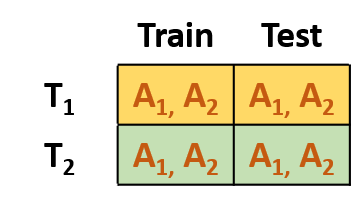
\includegraphics[trim=20 5 0 0 ,clip,width=.75\linewidth]{images/Picture3}
    \caption{Same-topic\label{Fig:scenarios.a}}
  \end{subfigure}%
  \hfill 
  \begin{subfigure}{0.33\textwidth}
  \centering
    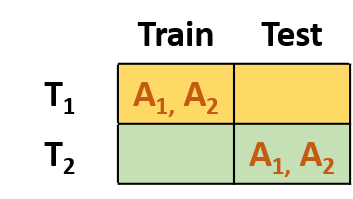
\includegraphics[trim=20 5 0 0 ,clip,width=.75\linewidth]{images/Picture1}
    \caption{Cross-topic\label{Fig:scenarios.b}}
  \end{subfigure}
  \hfill
  \begin{subfigure}{0.33\textwidth}
  \centering
    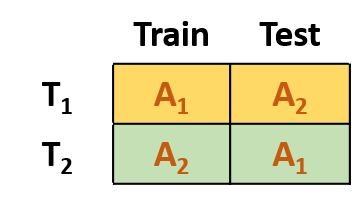
\includegraphics[trim=20 5 0 0 ,clip,width=0.75\linewidth]{images/Picture4}
    \caption{Topic-confusion (Proposed)\label{Fig:scenarios.c}}
  \end{subfigure}%
  \caption{Authorship attribution scenarios. (T: Topic, A: Author)\label{Fig:scenarios}}
\end{figure*}


\section{Related Work}

The first work that used a computational approach is~\citep{Mosteller.f:1964}, which used the Na\"ive Bayes algorithm with the frequency of function words to identify the authors of the Federalist papers~\citep{Juola.p:2008}. Research efforts have aimed at finding new sets of features for current domains/languages, adapting existing features to new languages or media, or using new classification techniques~\citep{f2007identifying,Iqbal.F:2013,Stamatatos.E:2013, Sapkota.U:2014,sapkota2015not,Ding.S:2015,malik:2018}. 

Recent attempts have been made to investigate authorship attribution in realistic scenarios, and many studies have emerged where the constraints differ from the training to the testing samples such as~\citep{bogdanova-lazaridou-2014-cross} on cross-language,~\citep{goldstein2009person,custodio2019ensemble} on cross-domain/genre, and finally,~\citep{sundararajan2018represents,Stamatatos.E:2017,stamatatos2018masking,Barlas2020,Barlas2021} on cross-topic.

\citet{Stamatatos.E:2017, stamatatos2018masking,Barlas2020,Barlas2021} achieved state-of-the-art results on cross-topic authorship attribution. 
\citep{Stamatatos.E:2017, stamatatos2018masking} proposed a character- and word- level $n$-grams approach motivated by text distortion~\citep{granados2012contextual} for topic classification. In contrast to~\citep{granados2012contextual}, ~\citeauthor{stamatatos2018masking} kept the most frequent words and masked the rest of the text.~\citet{Barlas2020,Barlas2021} explored the widely used and massively pretrained transformer-based~\citep{vaswani2017attention} language models for authorship attribution. Specifically, they trained a separate language model for each candidate author with a pretrained embeddings layer from ELMo~\citep{peters-etal-2018-elmo}, BERT~\citep{devlin2019bert}, GPT-2~\citep{radford2019language} and ULMFit~\citep{howard2018universal}. Each model was presented with words from the investigated document, and the most plausible author for that document is the one whose model has the lowest average perplexity.

\begin{figure}[hbt!]
    \begin{subfigure}{0.24\textwidth}
    \centering
    % % 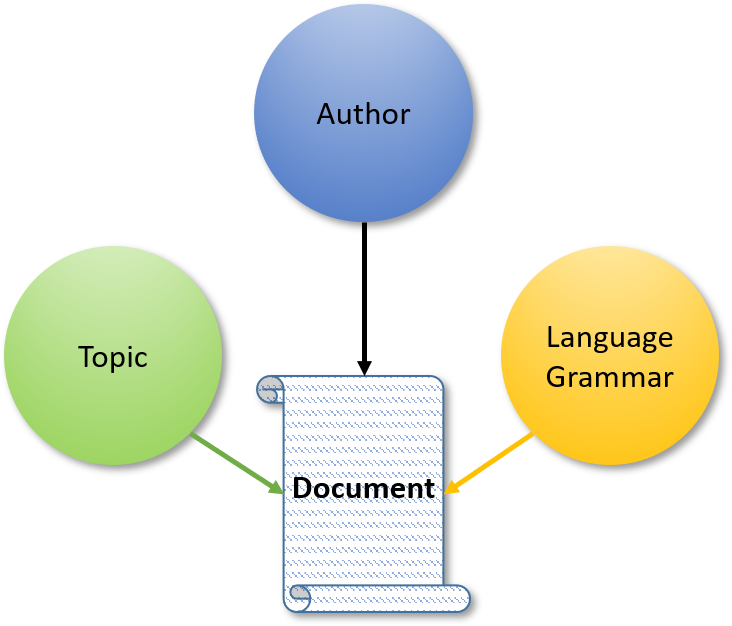
\includegraphics[width=0.50\textwidth]{images/causal_old}
    % \includegraphics[width=.9\textwidth, trim={0.15cm 0 6.4cm 0},clip]{images/relationdiagram}
    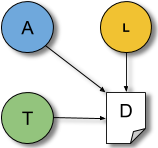
\includegraphics[width=\textwidth]{images/relationdiagram_a}
    \caption{Assumed.\label{causal.perc}}
    \end{subfigure}~
    % \hfill
    \begin{subfigure}{0.24\textwidth}
    \centering
    % % 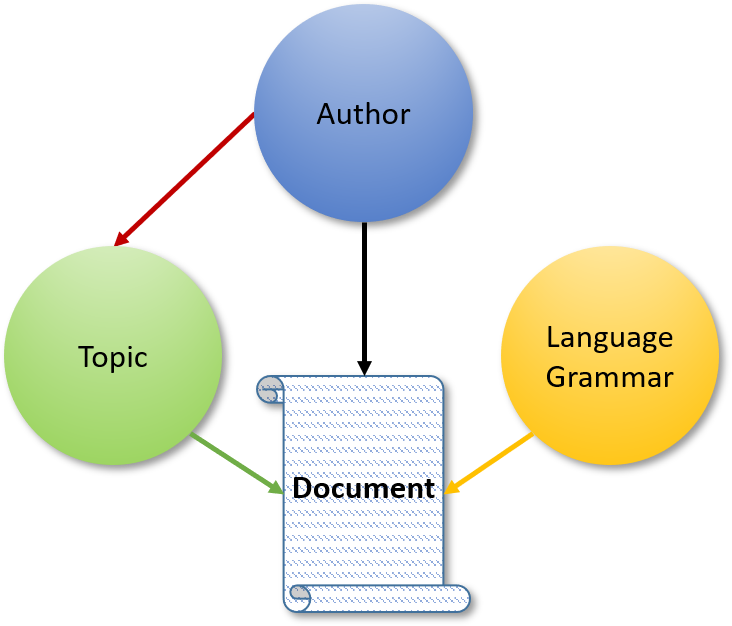
\includegraphics[width=0.50\textwidth]{images/causal} 
    % \includegraphics[width=.9\textwidth, trim={6.5cm 0 0cm 0},clip]{images/relationdiagram}
    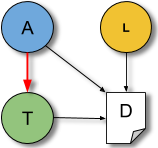
\includegraphics[width=\textwidth]{images/relationdiagram_b}
    \caption{Proposed.\label{causal.prop}}
    \end{subfigure}
%   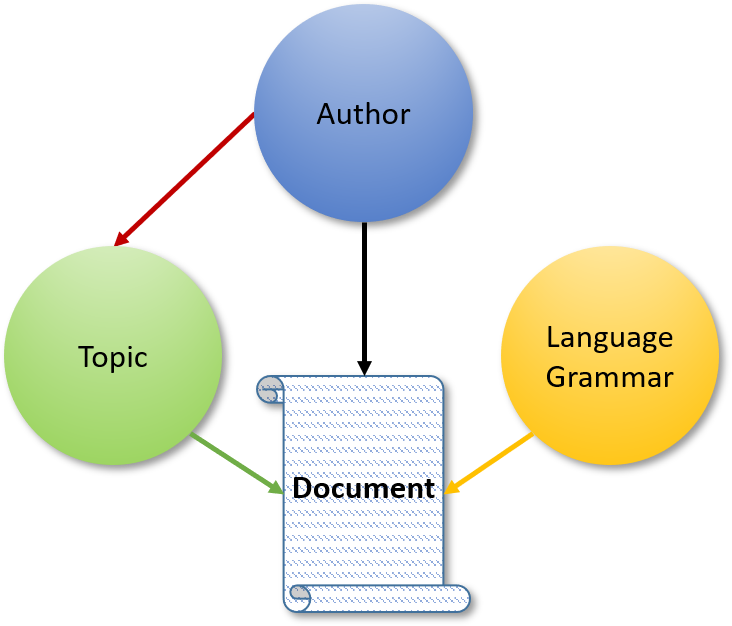
\includegraphics[width=0.25\textwidth]{images/causal.png} % first figure itself
  \caption{The relationship diagram between the topic (T), the author's style (A), the language (L), and the document (D).}
  \label{fig:causal}
\end{figure}
\section{The Topic Confusion Task\label{sec:confTask}}
\subsection{Theoretical Motivation}
\begin{figure*}[htb!]
    \centering
    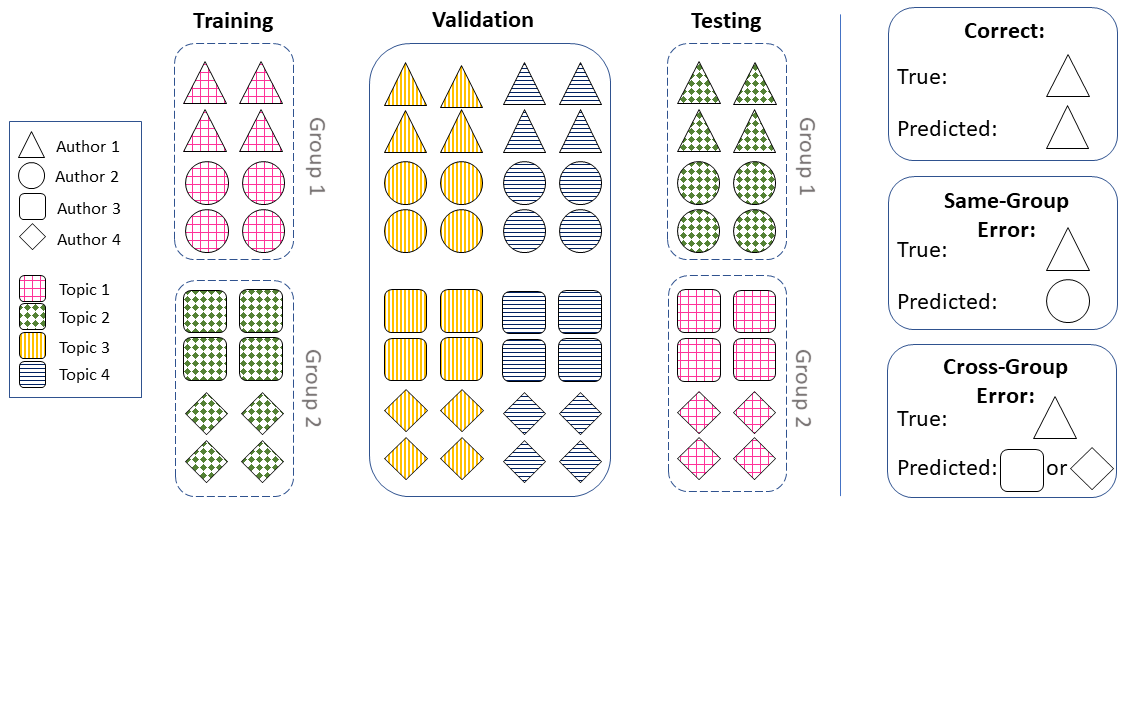
\includegraphics[width=.99\textwidth, trim={0 5.5cm 0 0},clip]{images/Presentation1.png}
    \caption{Topic confusion task. We use two topics for training and switch them for testing. Two topics are used for hyperparameter tuning. The topic labels are not available for the classifier during training, and are only used to distribute the samples over the subsets and calculate the scores.}
    \label{fig:topicConf}
\end{figure*}

Figure~\ref{causal.perc} shows the assumed relationship diagram between a document, its author, its topic, and the language rules\footnote{There could be other unknown factors that affect any random variable which the attribution process is not aware of.} that govern the writing process~\citep{Ding.S:2019}. According to~\citet{Ding.S:2019}, these are the factors that affect the process of writing a document. Given a topic's distribution over words, the author picks a subset of these words and connects them using the language rules which govern what words accompany these topical words and how sentences are structured. Eq.~\ref{Eq.Joint} shows the joint probability while ignoring the language model, and assuming the topic distribution is independent from that of the author. 
\begin{flalign}
    P(A, T, D) \phantom{xx} &= P(A)P(T)P(D|A,T) \hfill \label{Eq.Joint}\\
    P(A=a|D) \phantom{x}  &\propto \sum_{t}^{T} \left[ 
    P(A=a)P(T=t)\nonumber \right. \\
     & \left. \phantom{xxxxx} P(D|T=t, A=a) \right] \hfill
    \label{Eq.cond}
\end{flalign}
During the attribution process, the model is used to predict an author given an anonymous document using Eq.~\ref{Eq.cond}, which follows from Eq.~\ref{Eq.Joint} after applying Bayes rule. The same argument about the topic also applies to the language model, but for simplicity, we only focus on the topic since POS tags have been shown to capture the stylistic variations in language grammar between authors.

Same-topic scenarios assume that the document generation depends only on the author's writing choices, completely ignoring the topic; i.e., no $T$ in the joint distribution, and so, $P(A=a|D)$ is $\propto P(A=a)P(D|A=a)$, but this is unrealistic and unintuitive. In contrast, cross-topic scenarios account for the topics' effects but they assume that the topic is independent from the author. This is clear from the cross-topic setup where the topic values are fixed during training and testing. While this setup highlighted an critical flaw in same-topic scenarios and encouraged classification models to rely less on the topic to do authorship attribution, it does not help in identifying the causes of the errors that resulted from changing the topic between training and testing. 

Instead, we propose a setting in which the topic is dependent on the author, as shown in Figure~\ref{causal.prop}, but this dependence varies between training and testing. Our intuition about the effect of the author's writing style on the topic is the following. Consider a topic that has a unique word distribution which can be captured by analyzing a fairly large corpus of documents on that topic. An author writing on that topic will likely generate a slightly different distribution in their document because the limited document's length will force an author to choose a subset of words that describe that specific topic. This topic distribution will also differ across documents written by different authors because words have synonyms and the same idea can be worded in multiple ways. 

If we allow the topic to depend on the author, then the joint distribution changes from Eq.~\ref{Eq.Joint} to~Eq.~\ref{Eq.Joint2}, and the conditional probability of an author given the anonymous document will change to Eq.~\ref{Eq.cond2}.
%
\begin{flalign}
    P(A, T, D) \phantom{xx} &= P(A)P(T\textcolor{blue}{|A})P(D|A,T) \hfill \label{Eq.Joint2}\\
    P(A=a|D) \phantom{x} &\propto \sum_t^{T} \left[ P(A=a)  P(T=t\textcolor{blue}{|A=a}) \right. \nonumber \\
    & \left. \phantom{xxxxx} P(D|T=t, A=a) \right]  
    \label{Eq.cond2}
\end{flalign}

Because we allow the topic to depend on the author, we can create a scenario where a learning algorithm only sees samples on one topic for a specific author in the training set but a different topic in the test set, then we measure the error caused by this switch. Note that this proposed scenario will not be as easy as the same-topic, introduces new topics at test time, and can help us understand the entanglement of the topic and the writing style.

\subsection{The Proposed Setup\label{subsec:proposed}}
Compared to the standard cross-topic setting, this task can help us understand how the topic affects certain features by showing whether the error is caused by the topic or the features themselves, while the cross-topic setting would give a more realistic performance compared to the same-topic, but without any insights on why we got such results.

We propose a new task to measure the performance of authorship attribution techniques given a confounding topic--author setting. The key characteristic of this task is how we associate the topics and the authors in the training, validation and testing sets. Given a set of writing samples written by $N$ authors on $T$ topics where the number of authors $N \geq 4$, the number of topics $T \geq 3$, and each author has, approximately, the same number of writing samples on each topic $T$. 

First, we divide the authors into two equal-sized groups: group 1 and group 2. Next to create the training set, we select two random topics and use writing samples on topic 1 for the authors in group 1 and writing samples on topic 2 for the authors in group 2. For the testing set, we flip the topics configuration that we used for the training set. We use writing samples on topic 2 (instead of 1) for the authors in group 1 and samples on topic 1 (instead of 2) for the authors in group 2. Finally, we use the remaining writing samples on the unused topics for the authors in both groups for the validation set. Figure~\ref{fig:topicConf} shows the setup for the proposed task as an example of having four authors and four topics.

After creating the training, validation, and testing sets, we train models for authorship attribution. First, the features are extracted from the writing samples. Second, a classification model is trained on the training samples, tuned on the validation set to pick the best hyperparameters, and tested on the testing set. Note that the classifier does not have access to any information about the setup, such as the groups configuration or the topic labels. 

The advantage to this setup is that, we can sub-divide the errors that the model makes on the validation and test sets. In particular, we count the following cases:

\noindent$1.$ \textbf{Correct (\%)}: The number of correctly classified samples divided by the total number of predicted samples.

\noindent$2.$ \textbf{Same-group error (\%)}: The number of misclassified samples to authors within the same group as the true author divided by the total number of predicted samples.

\noindent$3.$\textbf{Cross-group error (\%)}: The number of misclassified samples to authors in the other group divided by the total number of predicted samples.

Distinguishing these types of errors allows us to investigate whether features in a classifier tend to be indicative of writing style or topic. In particular, features that are invariant to the topic and only capture the authors' writing styles should lead a model to correctly identify the author in the test set. Conversely, features that capture the topic instead of the writing style would lead a model to classify according to topic, resulting in cross-group errors. Finally, a model that fails for other reasons---either because the writing styles are too similar or because the used features can only partially capture the writing styles---will misclassify samples to authors within the same group.

% Compared to the standard cross-topic setting, this task can help us understand how the topic affects certain features by showing whether the error is caused by the topic or the features themselves, while the cross-topic setting would give a more realistic performance compared to the same-topic, but without any insights on why we got such results. 

\section{Dataset\label{subsec:dataset}}
We present an extended, curated, and relatively balanced version of the Guardian dataset.\footnote{Appendix~\ref{dataColl} describes the data collection procedure, which documents were excluded and the reason for exclusion, a list of the articles URLs, and the code to scrape and preprocess the articles to the format which we used.} One motivation is that as we try to understand the effect of the topic on the attribution process, we need to isolate any external factors that may affect the performance and make the results noisy. For example, in the topic confusion task, we have to use topics with writing samples from all the authors. Otherwise, the model could learn to favour one topic versus the other during training, while on test time, it will have author samples that it did not see during training. Based on that, it will be hard to tell whether these samples will be misclassified due to lack of training samples or due to a strong topic effect on the attribution process. Although datasets in real life can be imbalanced, this issue can be addressed by randomly excluding some writing samples to make the dataset imbalanced or using proper performance metrics for imbalanced datasets such as weighted accuracy, precision, recall and F-Score. 

The number of collected articles is provided in Table~\ref{tab:myData_short}. Descriptive statistics are provided in Appendix~\ref{additional}, Table~\ref{tab:myData}.
\begin{table}[ht]
\caption{The number of articles per topic and per author in our dataset. (* Has less than 10 articles/author)}
    \label{tab:myData_short}
    \centering
    \begin{tabular}{ll |ll }
    \hline 
    \multicolumn{2}{l}{\textbf{$\#$ of articles/author}}   & \multicolumn{2}{|l}{\textbf{$\#$ of articles/topic}}  \\
    % \textbf{per author}          &   & \textbf{per topic} \\
    \hline
     M.K.                & 35   &  Politics (P) & 130 \\ 
     H.Y.                & 37   &  Society (S)  & 118*  \\
     J.F.                & 38   &  UK (U)       & 130    \\
     M.R. and P.P.       & 39   &  World (W)    & 130    \\
     \textbf{The remaining 8}   & 40 & & \\
     \hline
     \end{tabular}
\end{table}

\section{Authorship Attribution Models\label{subsec:QWS}}
In this section, we discuss two groups of authorship attribution models. The first group contains a set of classical models that use hand-engineered features and a classification algorithm. The second group comprises a set of neurally-inspired models motivated by recent advancements in various natural language processing tasks. Such models are considered end-to-end system where the feature representation is done as part of the model as opposed to being hand-crafted and provided to the model. 


\subsection{Classical Features with SVM} 
This approach approach uses a set of classical, hand-engineered features with a non-neural classification algorithm. We experiment with a wide spectrum of features that include both stylometric features and $n$-gram features. Early work on authorship attribution proposed using stylometric features to represent an author's writing Style. On the other hand, $n$-gram features were used with most text classification tasks until recent neural representations replaced them.

With all the following features, we used the instance-based approach~\citep{Stamatatos.e:2009} where a writing style is extracted from every sample separately. A classification model is trained on the extracted features to predict the authors of new, unseen samples. We used~\citet{scikit-learn}'s implementation of linear Support Vector Machines (SVM) as the classification algorithm\footnote{Appendix~\ref{appOptimal}, Tables~\ref{hypers} and~\ref{optimalTable} show the range of values and the average optimal parameters that are fine-tuned on the validation set, respectively.}, which is a common choice in authorship attribution~\citep{Stamatatos.E:2017}. 

Common classification 

Note that the literature has thoroughly compared and contrasted the performance of different classification techniques such as Na\"ive Bayes, decision trees and SVM~\citep{Ding.S:2015, malik:2018} with different kernels. This, therefore, is excluded from our work.   

\paragraph{Stylometric Features~\citep{Iqbal.F:2008,Iqbal.F:2013}.}
We evaluate 371 features including syntactic features and lexical features on both character- and word-level. These features are listed in Appendix~\ref{styloFeat}-Table~\ref{tbl:features}.

\paragraph{Character-, Word- and POS-level N-Grams~\citep{Stamatatos.E:2013,Sapkota.U:2014,sapkota2015not}.}
Using $n$-grams is a common approach to represent documents in authorship attribution. In most text classification tasks, the tokenization is done on either the word or the character level. We use both character and word level $n$-grams in addition to POS-level~\footnote{We used the POS tagger from~\citep{manning2014stanford}.} $n$-grams which are proven to be an essential indication of style~\citep{Ding.S:2015,sundararajan2018represents}. 

\paragraph{Masking~\citep{Stamatatos.E:2017,stamatatos2018masking}.}
This preprocessing technique replaces every character in words to be masked with a (*) and replaces all the digits with a ($\#$). Masked words are chosen based on their frequency in the British National Corpus (BNC), an external dataset. After Masking, tokens are put back together to recreate the original document structure before extracting $n$-gram features. 

\paragraph{Combining features.} One advantage to using hand-engineered features on the sample level is that these features can easily be combined. First, we evaluated the combination of the stylometric features and POS $n$-grams. Next, we combined both these features to the other classical features mentioned above. 


\subsection{Pretrained Language Models}

\paragraph{Few-Shot BERT and RoBERTa.}
This is an example of a few-shot classification with pretrained language models. We used a sequence classification model with a pretrained embeddings layer from the transformer-based non-autoregressive contextual language models BERT~\citet{devlin2019bert} and RoBERTa~\citep{liu2019roberta} followed by a pooling layer then a classification layer. Given the huge size of these models and the small number of training samples, we decided to freeze the embeddings and train only the classification layer. We used the implementation provided by the HuggingFace~\citep{Wolf2019HuggingFacesTS} library\footnote{\url{https://huggingface.co}}.

\paragraph{Author Profile (AP) BERT and RoBERTa~\citep{Barlas2020,Barlas2021}.} 
We trained a separate neural language model for each author in the dataset where the embedding layer is initialized with embeddings from BERT and RoBERTa. To predict the author, we used each language model --or author profile-- to calculate the average perplexity of the model for an investigated document. Before attribution, however, the perplexity scores are normalized using a normalization vector ($n$) to make up for the biases in the output layer of each language model, where $n_i$ equals the average perplexity of profile $A_i$ on the normalization corpus.

\citet{Barlas2020,Barlas2021} used two normalization corpora during inference: the training set (K) and the testing set without labels (U). The author with the lowest normalized perplexity score is the most plausible author of the investigated document. Note that assuming the availability of a test set rather than a single document is unrealistic in authorship attribution even if labels were not provided. We evaluated both cases for the sake of completeness.  

\section{\label{subsec:eval}Evaluation Procedure}
For each set of features, we used the setup explained in Section~\ref{sec:confTask} to create a 100 different configurations. For each configuration, we randomly ordered the topics, selected 12 out of the 13 available authors, and distributed the authors to the groups. This setting is considered as one single experiment. To account for randomness in the classification algorithm, we repeated every single experiment ten times\footnote{We trained FS BERT and FS RoBERTa only once.}, and reported the average balanced accuracy score and standard deviation.

We decided to omit one author and use the remaining twelve out of the available 13 authors to balance the groups. With this split, the probability of picking the correct author is $\frac{1}{12}$, the likelihood of choosing a wrong author in the same group is $\frac{5}{12}$, and the probability of picking a wrong author in the other group is $\frac{6}{12}$. This case applies if the true author was in either group 1 or group 2. However, suppose we were to use all the 13 authors and divide them into two groups of six and seven authors, respectively. In that case, the probabilities will differ depending on whether the actual author is in the group with six authors or seven authors. In that case, we will need to re-weight the errors based on their probability, and that will complicate the results as we will not be talking about the exact number of samples.  

\begin{table*}[htb]
\centering
\caption{\label{tbl:topicConf}Results (\% $\pm$ SD) on the topic confusion task and the cross-topic scenario. The first row of each group of rows corresponds to an existing method. The last row is random performance. (\textbf{Boldface}: best result per column. $\uparrow$ Higher is better. $\downarrow$ Lower is better. \%: Percentage. \textcolor{red}{$^{*}$}State of the art. \textcolor{red}{$^{**}$} Has access to the (unlabeled) test set.)
}
\begin{tabular}{l|ccc|||c}
\hline
& \multicolumn{3}{c|||}{\textbf{Topic Confusion}}& \textbf{Cross-topic}    \\\hline
\multirow{2}{*}{\textbf{Models}}  & $\uparrow$ \textbf{Correct} & $\downarrow$ \textbf{Same-group} & $\downarrow$ \textbf{Cross-group} & \textbf{$\uparrow$ Accuracy} \\
 &  & \textbf{Error} & \textbf{Error} &   \\\hline\hline 
 
 Stylo. &   73.8 $\pm$ 4.9 & 18.3 $\pm$ 3.2 & 24.8 $\pm$ 3.5 &  61.2 $\pm$ 3.1\\\hline
 POS $n$-grams &	84.2 $\pm$ 5.3& 13.4 $\pm$ 3.4	& 	19.4 $\pm$ 3.9& 71.0 $\pm$ 3.2\\
\phantom{hi} + Stylo       & 93.1 $\pm$ 4.7&   9.8 $\pm$ 3.0 & 14.1 $\pm$ 3.3 & 79.2 $\pm$ 2.7  \\\hline
						
 Char $n$-grams  & 82.0 $\pm$ 7.6 & 7.9 $\pm$ 2.8 & 27.1 $\pm$ 7.6 & 77.3 $\pm$ 2.8 \\			
 \phantom{hi}+ Stylo & 85.4 $\pm$  7.5& 7.6 $\pm$ 3.0 & 24.0 $\pm$ 7.1 & - \\
\phantom{hi}+ Stylo \& POS & 89.8 $\pm$ 7.1 & \textbf{7.0} $\pm$ 2.7 & 20.1 $\pm$ 6.5 & 82.8 $\pm$ 2.7\\\hline

 Word $n$-grams & 73.1 $\pm$ 8.6 & 9.3 $\pm$ 3.2 & 34.6 $\pm$ 8.6 & 77.7 $\pm$ 2.7\\
 \phantom{hi}+ Stylo & 84.7 $\pm$ 7.5 & 8.5 $\pm$ 2.7 & 23.8 $\pm$ 7.2 & - \\
 \phantom{hi}+ Stylo \& POS  & 93.9 $\pm$ 5.8 & 8.3 $\pm$ 3.1 & 14.7 $\pm$ 4.9 & \textbf{83.3} $\pm$ 2.6\\
\hline
			
  Masking (Ch.)\textcolor{red}{$^{*}$} & 92.9 $\pm$ 6.5 & 7.9 $\pm$ 3.2 & 16.1 $\pm$ 5.8  & 80.9 $\pm$ 2.6\\
  \phantom{hi}+ Stylo \& POS & 97.2 $\pm$ 5.6 & 7.5 $\pm$ 3.2 & 12.2 $\pm$ 4.1 & 83.2  $\pm$ 3.3\\\hline

 Masking (W.)  & 89.8 $\pm$ 6.7 & 9.3 $\pm$ 3.4 & 17.9 $\pm$ 6.7 & 77.9 $\pm$ 4.0\\
 \phantom{hi}+ Stylo \& POS & \textbf{97.5} $\pm$ 5.2 & 7.8 $\pm$ 3.2 & \textbf{11.7} $\pm$ 3.7 & 82.8 $\pm$ 3.3\\

\hline \hline
 FS BERT   & 38.7 $\pm$ 6.7 & 23.3  $\pm$ 6.6 & 55.0  $\pm$ 10.5 & 37.5 $\pm$ 3.5\\
 BERT AP (K) & 60.3 $\pm$ 8.8 & 9.6 $\pm$ 3.6 & 47.0 $\pm$ 10.0 & 67.3 $\pm$ 4.4\\
 BERT AP (U\textcolor{red}{$^{**}$}) & 60.9 $\pm$ 8.5 & 9.8 $\pm$ 3.7 & 46.3 $\pm$ 10.0 & 71.1 $\pm$ 3.3\\

\hline
 FS RoBERTa & 46.6 $\pm$ 8.8 & 15.3 $\pm$ 6.0 & 55.1 $\pm$ 12.7 & 51.1 $\pm$ 3.4\\
 RoBERTa AP (K) & 67.6 $\pm$ 8.3 & 8.3 $\pm$ 3.4 & 41.0 $\pm$ 9.9 & 70.8 $\pm$ 2.0\\
 RoBERTa AP (U\textcolor{red}{$^{**}$}) & 68.9 $\pm$ 8.3 & 8.0 $\pm$ 3.3 & 40.1 $\pm$ 9.7 & 75.8 $\pm$ 3.8\\

\hline\hline
 \multirow{1}{*}{\textit{``random chance"}} & 9.4 & 48.7 & 58.5 & 7.7\\\hline
\end{tabular}

\end{table*}

\section{Results and Discussion}
\subsection{Topic Confusion Task}
Table~\ref{tbl:topicConf} shows the results on the topic confusion task using the proposed measured in section~\ref{subsec:proposed}. Correct is the percentage of samples that were correctly classified, same-group error is the percentage of samples that were attributed to the wrong author but within the same group as the correct author, and finally cross-group error is the percentage of samples that were attributed to the wrong author and to the author group that does not contain the correct author ---caused by the change in the topic---. 

We start by comparing the standard features in authorship attribution: (1) stylometric vs. (4) character- and (7) word-level $n$-gram features. We see why stylometric features were out-favoured by $n$-gram features if we look only at the accuracy. Character $n$-grams achieve higher accuracy while word-level $n$-grams perform similarly but are easier to collect and do not require adapting between different languages or media. However, splitting the error shows that stylometric features have the lowest cross-group error caused by the topic shift. The topic shift does not cause the low performance of stylometric features but rather because they partially capture the writing style.

When looking at (4) character- vs (7) word-level $n$-grams, we see that they have comparable same-group errors while cross-group error is much higher for word $n$-grams. Our results are in line with the literature on the classical cross-topic authorship scenario, which shows that character $n$-grams outperform word $n$-grams while still capturing the topic, which makes character $n$-grams less influenced by the topic in the attribution task.

Furthermore, all the classical features (1, 2, 4, and 7) Part-Of-Speech $n$-grams have the highest accuracy and the lowest topic bias (cross-group error). This outcome is intuitive as POS tags are not content words. Still, their same-group error is higher than character- and word-level $n$-grams, which explains why researchers preferred $n$-gram features over them for authorship attribution.  

Next, we look at the effect of masking as a preprocessing technique. Specifically, we compare character- and word-level $n$-gram features before (4 and 7) and after masking (10 and 12). Masking infrequent words is evident in the cross-group error between character $n$-grams and masking on the character-level as well as the word $n$-grams and masking on the word level. Table~\ref{tbl:topicConf} shows the same-group error remained fixed while cross-group error decreased by 11 and 17 samples for the character- and the word-level, respectively. 

% \paragraph{Combining features.} One advantage to using hand-engineered features on the sample level is that these features can easily be combined. First, we combined the stylometric features and POS $n$-grams and observed (3) a decrease in both same- and cross-group errors, which translates to better writing style representation and lower topical bias. 

Next, we evaluated the effect of combining both stylometric features and POS $n$-gram features with character- and word-level $n$-grams with and without masking (rows 6, 9, 11, and 13). The results of combining both stylometric features and POS $n$-grams with all the other features have decreased the cross-group error significantly, which resembles less confusion over the topic. On the other hand, the same-group error was reduced by merely one sample at max in most cases. 

It is worth noting that masking on the character level performed better than masking on the word level without any additional features. In contrast, when stylometric features and POS $n$-grams are added to both masking approaches, the word-level masking performs better.

\paragraph{Pretrained Language Models.} These models performed very poorly on this topic confusion task (rows 14 to 19) regardless of the attribution approach being used with them. In all cases, the same-group error representing the capacity to capture the writing style was on par with character- and word-level $n$-grams, while the cross-group error is double in some cases. 

Indeed, pretrained neural language models are not suited for authorship attribution. Their goal is to learn word representations that capture the similarity between words that appear in a similar context, something that one-hot encoding does not capture. In authorship, however, words must both appear in the same context and be used by that author to have similar representations. For example, `color' and `colour' are the same word but with different spelling based on whether American or British English is being used. Ideally, these two words would have very similar embeddings, if not identical ones. The distinction between the two is critical because it indicates the author's identity or the language system they use. Authorship attribution techniques highlight these differences and use them to identify the most plausible author of an anonymous document. 

\subsection{Comparing the Performance on the Cross-Topic Scenario}
To validate our findings in a realistic scenario, we compare the performance in the cross-topic scenario on the Guardian dataset. Note that it is common to do the evaluation on one of the two cross-topic authorship attribution datasets~\citep{goldstein2009person,Stamatatos.E:2013} similar to~ \citep{goldstein2009person,Sapkota.U:2014,Stamatatos.E:2017, stamatatos2018masking,Barlas2020,Barlas2021}

% \begin{table}[htb]
% \caption{\label{tbl:Xtopic}Results on the traditional, cross-topic scenario. \textbf{Boldface} indicates the best result per column. ($\uparrow$ Higher is better. \textcolor{red}{$^{*}$}State of the art. \textcolor{red}{$^{**}$} Has access to the (unlabeled) test set.)}
% \centering
% \begin{tabular}{l|l|c }
% \hline
% \multicolumn{3}{c}{\textbf{Cross-topic}}    \\\hline
% \# & \textbf{Models} & \textbf{Accuracy (\%) $\uparrow$ } \\\hline
% 1) & Stylo                & 61.2 $\pm$ 3.1\\\hline

% 2) & POS $n$-grams   & 71.0 $\pm$ 3.2\\
% 3) & \phantom{hi}+ Stylo         & 79.2 $\pm$ 2.7\\\hline

% 4) & Char $n$-grams   & 77.3 $\pm$ 2.8\\
% % \phantom{hi}+ Stylo  & - \\
% 5) & \phantom{hi}+ Stylo \& POS   & 82.8 $\pm$ 2.7\\\hline

% 6) & Word $n$-grams   & 77.7 $\pm$ 2.7\\
% % \phantom{hi}+ Stylo   & - \\
% 7) & \phantom{hi}+ Stylo \& POS    & \textbf{83.3} $\pm$ 2.6\\\hline

% 8) & Masking (Ch.)\textcolor{red}{$^{*}$}      & 80.9 $\pm$ 2.6\\
% 9) & \phantom{hi}+ Stylo \& POS  & 83.2  $\pm$ 3.3\\\hline

% 10) & Masking (W.)    & 77.9 $\pm$ 4.0\\
% 11) & \phantom{hi}+ Stylo \& POS    & 82.8 $\pm$ 3.3\\
% \hline
% 12) & FS BERT  & 37.5 $\pm$ 3.5\\
% 13) & BERT AP (K) & 67.3 $\pm$ 4.4\\
% 14) & BERT AP (U\textcolor{red}{$^{**}$}) & 71.1 $\pm$ 3.3\\
% \hline
% 15) & FS RoBERTa  & 51.1 $\pm$ 3.4\\
% 16) & RoBERTa AP (K) & 70.8 $\pm$ 2.0\\
% 17) & RoBERTa AP (U\textcolor{red}{$^{**}$}) & 75.8 $\pm$ 3.8\\
% \hline
% \hline
% & \multirow{1}{*}{\textit{``random chance"}}   & 7.7 \\\hline
% \end{tabular}
% \end{table}

Table~\ref{tbl:Xtopic} shows that a combination of stylometric features, POS- and word-level $n$-grams (7), outperforms the state-of-the-art, which is (8) masking the least frequent words followed by word-level $n$-gram features. Adding stylometric features and POS-level $n$-grams to (9) masking (Ch) and (11) masking (W) also achieved better performance than state of the art. Still, the difference was statistically significant only when we compared (8) masking (Ch.) and (7) ($P=0.04$). Appendix~\ref{additional} contains the experimental setup, detailed results and analysis supported with statistical significance tests and an ablation study on the cross-topic scenario.

It is essential to highlight how current results do not shed light on the capacity of features. Table~\ref{tbl:Xtopic} shows similar accuracy scores for different techniques. Conversely, the topic confusion task reveals completely different behaviour for each feature. 

\section{Conclusion}
In this work, we proposed the topic confusion task, which helps test the capacity of features in capturing the writing style while being influenced by the topic in authorship attribution. Additionally, it could help in understanding the cause of the errors in authorship attribution. We verified the outcomes of this task on the cross-topic authorship attribution scenario. We showed that a simple linear classifier with stylometric features and POS tags could improve the authorship attribution performance compared to the commonly used $n$-grams. We achieved a new state-of-the-art of 83.3\% on the cross-topic scenario by resurrecting stylometric features and combining them with POS tags and word-level $n$-grams, 3\% over the previous state-of-the-art, masking-based, character-level approach. When neurally-inspired techniques are very appealing in all domains, we showed that the simple, hand-crafted stylometric features combined with POS tags better capture the writing style than these pretrained language models. 

% \section*{Acknowledgments}
% The acknowledgments should go immediately before the references.  Do
% not number the acknowledgments section. Do not include this section
% when submitting your paper for review. \\

\newpage
\section{Ethics/Broader Impact Statement}
\subsection{Data Collection}
\noindent$\bullet$ The data collection process is described in Appendix~\ref{dataColl}. Scripts to retrieve the articles are also provided in the supplementary material. As per the requirements of the Guardian API, we do not share the actual articles, but rather the URLs and the script to extract the original articles. In addition to ownership rights, this is important in case the original authors of these articles decide to delete them, or make some modifications to these articles. The articles that we use are available online, and do not discuss sensitive topics that, if shared, could hurt the original authors of these articles. 

\noindent$\bullet$ All the \textbf{manual work} that was required, such as removing the authors names from the body of the articles, was done solely by the authors. No external/paid help was required. Details of all the manual work is provided in the supplementary material (not the Appendix). To ensure reproduciblity of this manual work, we provided a list of all the steps and how to perform them. 

\noindent$\bullet$ To ensure the \textbf{quality of the dataset}, we manually inspected the documents for potential features that would reveal the identity of the authors easily. The dataset has 508 documents which makes the task of manually inspecting the documents tedious, but possible. Future work does not need to do this inspection. We provide a list of all the required manual changes in the supplementary material. 

\subsection{Applications}
\noindent$\bullet$ \textbf{The intended use of this work.} One application of authorship attribution is in crime investigation where a domain expert can help law enforcement identify the true author of an anonymous investigated text. This anonymous text can be a threatening message, or a suicide note. In the famous case of Ted Kaczynski, also known as the ``Unabomber", linguistic evidence was used to identify Kaczynski by comparing his PhD thesis to the communication letters and the ``manifesto" sent to the investigating authorities by the Unabomber. 

Another area that could benefit from this work is research on anonymization, which is the task of hiding the identity of an author of a document to protect their privacy. To evaluate anonymization techniques, their outcome, i.e., the anonymized documents, are presented to an authorship attribution technique to identify their original author after anonymization. The effectiveness of these anonymization techniques is based on the change in the attribution accuracy before and after anonymization. As this work aims to provide a better understanding of what makes a writing style, we hope that this would lead to better anonymization techniques. 

Finally, it is important for the public to know about the existence of such authorship techniques which can identify them using small number of their writing samples. They need to know that their identities are not completely protected by the anonymity of the internet. If a small research group can develop such techniques, then governments and organizations with more budget and personnel can do the same or more, if they intend to. 

\noindent$\bullet$ \textbf{Failure mode} is exactly what we try to address in this work. Current authorship attribution techniques are highly affected by the topic of the documents, hence the outcome of the attribution process could potentially pick the wrong candidate due to topic similarity between the author's writing samples and the investigated document, and not the actual writing style. 

\noindent$\bullet$ \textbf{Potential misuse} can occur if this work is used against people who benefit from the internet anonymity to express their opinions against oppressing governments or individuals. In this case, individuals or governments would use the same techniques to identify people who speak against their interests, and persecute them. 
\newpage
% Entries for the entire Anthology, followed by custom entries
\bibliography{tallip}
\bibliographystyle{acl_natbib}

\appendix

\onecolumn

\section{Data Collection\label{dataColl}}
First, we curated the existing dataset by retrieving the 381 original documents from the Guardian's website. Next, we inspected the authors' names and the topics associated with each article. We excluded the articles that had the wrong topic (e.g. labelled as ``Politics" in the dataset while having a ``Society" tag on the website), or the ones that appeared under more than one of the previous topics, or were co-authored by multiple authors. 

Next, we used the Guardian's API\footnote{\url{https://open-platform.theguardian.com}} to get all the articles written by each author, filtered them based on the topic, and collected the URLs of these articles and new articles aiming for 10 documents per author per topic. This resulted in a total of 40 documents per author. Note that while some authors have been writing in the Guardian for more than 20 years, they would mostly focus on one topic while occasionally writing on the other four. As a result, we still could not get 10 articles per author on the Society topic. The supplementary material contains full instructions, and the necessary script to get the data and preprocess it. We provide some descriptive statistics for the collected dataset in Table~\ref{tab:myData}. 
\begin{table*}[ht]
    \centering
    \begin{tabular}{ll |lll }
    \hline 
    \textbf{Total number of:} & &
    \multicolumn{2}{l}{\textbf{Number of articles per topic}} &
    \\\hline
    \phantom{Hi} Topics     & 4           & \phantom{Hi} Politics (P)  & 130            \\ 
    \phantom{Hi} Authors    & 13          & \phantom{Hi} Society (S)  & 118*          \\  
    \phantom{Hi} Articles   & 508         & \phantom{Hi} UK (U)      & 130           \\
    \phantom{Hi} Words      & 3,125,347   & \phantom{Hi} World (W)   & 130            \\
     \hline
     \textbf{Average number of: } & &
     \multicolumn{2}{l}{\textbf{Number of articles per author}} \\\hline
     \phantom{Hi} Articles / Author   & = 39.1 ($SD=1.5$)                         & \phantom{Hi} M.K.                & 35\\
     \phantom{Hi} Articles / Topic    & = 127 ($SD=5.2$)                          & \phantom{Hi} H.Y.                & 37\\
     \phantom{Hi} Words / Author      & $\approx$ 41 K ($SD$ $\approx$ 6.9 K)   & \phantom{Hi} J.F.                & 38\\
     \phantom{Hi} Words / Topic       & $\approx$ 781 K($SD$ $\approx$ 13.0 K)  & \phantom{Hi} M.R. and P.P.       & 39 \\
     \phantom{Hi} Words / Document    & $\approx$ 1050.2                        & \phantom{Hi} \textbf{The remaining 8}   & 40 \\ \hline
     \end{tabular}
    \caption{Descriptive statistics for the extended Guardian dataset (* Has less than 10 articles per author).}
    \label{tab:myData}
\end{table*} 

\section{Stylometric Features\label{styloFeat}}
\begin{table*}[htbp]
\centering
\begin{tabular}{p{7cm}}
\hline
\textbf{Lexical Features - Character-Level}  \\\hline
1. Characters count (N) \\
2. Ratio of digits to N \\
3. Ratio of letters to N \\
4. Ratio of uppercase letters to N \\
5. Ratio of tabs to N \\
6. Frequency of each alphabet (A-Z), ignoring case (26 features) \\
7. Frequency of special characters: \textless\textgreater\%\textbar\{\} []/$\backslash$@\#\~\ +-*=\$\^\ \&\_()' (24 features). \\
\end{tabular}
\begin{tabular}{|p{8cm}}
\hline
\textbf{Lexical Features - Word-Level}\\\hline
1. Tokens count (T)\\
2. Average sentence length (in characters)\\
3. Average word length (in characters)\\
4. Ratio of alphabets to N\\
5. Ratio of short words to T (a short word has a length of 3 characters or less)\\
6. Ratio of words length to T. Example: 20\% of the words are 7 characters long. (20 features)\\
7. Ratio of word types (the vocabulary set) to T\\
\end{tabular}\\
\begin{tabular}{p{15.5cm}}
\hline
\textbf{Syntactic Features}  \\\hline
1. Frequency of Punctuation: , . ? ! : ; ' " (8 features) \\
2. Frequency of each function words \citep{OShea.J:2013} (277 features)\\
\hline
\end{tabular}
\caption{List of stylometric features.\label{tbl:features}}
\end{table*}

\newpage
\section{Optimal Hyperparameters\label{appOptimal}}
\begin{table*}[htbp]
\centering
\begin{tabular}{c|l }
\hline
\textbf{Hyperparameter}  &  \textbf{Range}  \\ \hline
$k$ & 100, 200, 300, 400, 500, 1000, 2000, 3000, 4000, 5000 \\
$f_{t} $ & 5, 10, 15, 20, 25, 30, 35, 40, 45, 50 \\
$n_{ch}$ & 3, 4, 5, 6, 7, 8 \\
$n_{w}$ & 1, 2, 3 \\
$epochs$ & 2, 5 \\
$vocab\_size$ & 2000, 5000 \\
\hline
\end{tabular}
\caption{\label{hypers}
Hyperparameters for masking and $n$-gram based feature representations. $k$ is the threshold for masking, $n_{w}$ is the word-level and POS $n$-grams, $n_{ch}$ is the character-level $n$-gram, and $f_{t}$ is the minimum frequency threshold in the whole dataset.}
\end{table*}

For FS BERT and RoBERTa, we used the pretrained sequence classification models. These pretrained models do not have hyperparameters for the model structure, but only have pretrained configurations. We used the base uncased models, where base refers to the models' size (not large, and not distilled) and trained on all-lower-case text. For the training procedure, we used the following: AdamOptimizer, lr=0.1, Epochs=500, EarlyStopping(min\_delta=1e-3, patience=100). Despite the large Epoch value, most models would stop after less than 150 epochs.

We implemented~\citet{Barlas2020} ourselves. The code was made available online in a later version~\citet{Barlas2021}. We performed a gridsearch hyperparameter tuning for the number of epochs and the vocabulary size. For the topic confusion task, we used epochs=2 and vocab\_size=2000 based on the ablation studies on Bert reported in~\citet{Barlas2020}. 

\begin{table*}[htbp]
\centering
\begin{tabular}{l|ccrr}
\hline
\textbf{Method}   & \textbf{$k$} & \textbf{$n$} & \textbf{$f_{t}$} & Feat. \\
\hline
Masking (W.)                  & 1,616.7  & 1.9 & 7.9 & 3,265.8 \\ 
Masking (Ch.)                 & 1,691.7  & 5.5 & 18.8 & 6,416.3 \\ 
Stylometric + POS                      & -        & 1.3 & 31.3 & 484.2 \\ 
Stylometric + POS + $n$-grams (W.)  & -    & 2.0 & 12.5 & 2,481.0\\ 
Stylometric + POS + $n$-grams (Ch.) &   -      & 3.8 & 38.3 & 5,355.6\\ 
\hline
\end{tabular}
\caption{\label{optimalTable}
The average optimal parameters for each feature representation, with the resulting number of features under these settings ($k$: masking threshold, $n$: number of tokens in $n$-grams, \textit{$f_{t}$}: minimum frequency threshold in the dataset, W.: word-level, Ch.: character-level).}
\end{table*}

% \newpage


\counterwithout{subsection}{section}

\section{Additional Experiments\label{additional}}
\subsection{Data Splitting and Preprocessing\label{sec:prepro}}
% \begin{table}[ht]
%     \centering
%     \begin{tabular}{ll |lll }
%     \hline 
%     \textbf{Number of articles } & &
%     \multicolumn{2}{l}{\textbf{Number of articles}} & \\
%     \textbf{per author} & & \multicolumn{2}{l}{\textbf{per topic}} &
%     \\\hline
%      M.K.                & 35   &  Politics (P) & 130 \\ 
%      H.Y.                & 37   &  Society (S)  & 118*  \\
%      J.F.                & 38   &  UK (U)       & 130    \\
%      M.R. and P.P.       & 39   &  World (W)    & 130    \\
%      \textbf{The remaining 8}   & 40 & & \\
%      \hline
%      \end{tabular}
%     \caption{Additional details for the extended Guardian dataset (* Has less than 10 articles per author).}
%     \label{tab:fullmyData}
% \end{table}
\paragraph{The Cross-Topic Scenario.} In all our experiments, we split the dataset into training, validation and test sets. For the cross-topic experiments we followed the same setup in \citep{Stamatatos.E:2017}. We used one topic for training, another topic for validation and hyperparameter tuning, and the remaining two topics for testing. The number of articles was 127 articles when training on Society and 130 articles otherwise. This setup resulted in 12 different topics permutations. We reported the average overall accuracy on all the 12 configurations.

\paragraph{The Same-Topic Scenario.} We combined the 508 articles from all the topics, then split them as follows: 26\% for training, 26\% for validation, and the remaining 58\% for testing. This corresponds to 132 articles for training, 132 articles for validation, and 244 articles for testing. This ensures that the difference in performance between the same-topic and the cross-topic scenarios is not caused by the difference in the number of samples that are used for training/testing. We repeated this process 12 times and reported the average overall accuracy.

\subsection{Cross-Topic Authorship Attribution \label{sec:cross}}
As shown in Table~\ref{classification}, by combining the stylometric features and POS tags with $n$-gram features we achieve the highest accuracy of $83.3\%$. This is in line with our findings in the topic confusion task in Sec.~\ref{sec:confTask}. The difference between using all the features ($mean=83.26$, $SD=2.63$) and the character-based masking approach ($mean=80.89$, $SD=2.59$) is statistically significant ($P=0.04$)\footnote{We used a t-Test: Two-Sample Assuming Unequal Variances at the $\alpha = 0.5$ level.}. 

\begin{table*}[ht]
\parbox{.45\linewidth}{
\centering
\begin{tabular}{l|c|}
\hline
\textbf{Features}   & \textbf{Accuracy} \\
\hline
Stylo. + POS        & 79.2  $\pm$ (2.7)\\ 
Stylo. + POS +  $n$-grams (W.)   &  \textbf{83.3}  $\pm$ (2.6)\\ 
Stylo. + POS +  $n$-grams (Ch.)  &   82.8 $\pm$ (2.7)\\
Masking (W.)      & 77.9  $\pm$ (4.0)\\ 
Masking (Ch.)     & 80.9  $\pm$ (2.6)\\ 
Masking (W.) + Stylo. + POS      & 82.8  $\pm$ (3.3)\\
Masking (Ch.) + Stylo. + POS     & 83.2  $\pm$ (3.3)\\ 
FS BERT  & 37.5 $\pm$ (3.5)\\
BERT AP (K) & 67.3 $\pm$ (4.4)\\
BERT AP (U) & 71.1 $\pm$ (3.3)\\
FS RoBERTa  & 51.1 $\pm$ (3.4)\\
RoBERTa AP (K) & 70.8 $\pm$ (2.0)\\
RoBERTa AP (U) & 75.8 $\pm$ (3.8)\\
\hline
\end{tabular}
\caption{Average cross-topic classification accuracy (\%) on the extended Guardian dataset (W.: word-level, Ch.: character-level).\label{classification}}}
~~~~
\parbox{.45\linewidth}{
\begin{tabular}{|l|c}
\hline 
\textbf{Features} & \textbf{Accuracy}\\
\hline 
Stylo. &  61.2 $\pm$ (3.1)\\
POS & 71.0 $\pm$ (3.2)\\
W. $n$-grams & 77.7 $\pm$ (2.7) \\ 
Ch. $n$-grams & 77.3 $\pm$ (2.8) \\ 
Stylo. $+$ POS   &  79.2 $\pm$ (2.7) \\
Stylo. $+$ POS $+$ $n$-gram (W.) & \textbf{83.2} $\pm$ (2.6) \\
\phantom{Masking (Ch.) + Stylo. + POS}  & \\
\\\\\\\\\\\\
\hline
\end{tabular}
\caption{\label{ablatioin}
Ablation study: classification accuracy ($\%$) on cross-topic scenario. (Stylo.: Stylometric, W.: word-level)}}
\end{table*}

It is also worth noting that by using only stylometric features with POS $n$-grams we can achieve similar results to the masking approach with character-level tokenization. The difference of 1.7\% in favor of the masking approach is statistically insignificant ($P=0.15$) with a ($mean=80.89$, $SD=2.59$) for masking versus a ($mean=79.22$, $SD=2.70$) when using stylometric features with POS $n$-grams. 

Furthermore, Table~\ref{classification} shows a 3\% increase in the accuracy for the masking approach when using character-level tokenization. This outcome is in line with the findings in \citep{Stamatatos.E:2017}. The difference between word-level $n$-grams ($mean=77.90$, $SD=4.03$) and character-level ($mean=80.89$, $SD=2.59$) is statistically insignificant ($P=0.05$). Similarly, the difference between combining the stylometric features and POS-grams with word-level $n$-grams ($mean=83.26$, $SD=2.63$) versus with character-level $n$-grams ($mean=82.83$, $SD=2.7$) is statistically insignificant ($P=0.71$).

Finally, the difference between the state-of-the-art approach which is masking on the character-level from one side, versus stylometric features and POS tags combined with either character-level $n$-grams ($mean=80.89$, $SD=2.59$), masking on the word-level ($mean=82.80$, $SD=3.34$) or masking on the character-level ($mean=83.17$, $SD=3.33$) is statistically insignificant ($P=0.10$, $P=0.98$, and $P=0.80$, respectively.). The only statistically significant difference ($P=0.0.4$) was with stylometric features and POS tags combined with word-level $n$-grams ($mean=83.26$, $SD=2.63$)

\subsection{Ablation Study on the Cross-Topic Scenario\label{sec:abl}}
We conclude our experiments with an ablation study to see the contribution of each set of features to the overall accuracy. Similar to the experiments above, we perform a grid search over all the hyperparameters $f_t$ and $n$. As shown in Table~\ref{ablatioin}, each feature set on its own does not achieve the same performance as with combining all of them. We also confirm the previous results where, even in the cross-topic scenario, $n$-grams outperformed stylometric features by a large margin. We evaluated the significance of the difference between the top three accuracy groups. The results show that the difference between Set (3) ($mean=77.7$, $SD=2.69$) and Set (4) ($mean=79.3$, $SD=2.7$) is statistically insignificant ($P=0.21$) while it is significant ($P<0.01$) between Set (4) and Set (5) ($mean=83.3$, $SD=2.6$). 

% \subsection{Same-Topic Authorship Attribution\label{sec:same}}
% We experimented with the previously proposed features for the same-case scenario. Table~\ref{sameTopic} shows that, in line with the literature, $n$-gram based features outperform stylometric features which justifies why researchers considered them a good candidate for future representations. However, we show that combining them, as opposed to picking one versus the other can achieve higher accuracy than using each one of the separately.  
% \begin{table}[htbp]
% \centering
% \begin{tabular}{l|c}
% \hline
% \textbf{Method}   & \textbf{Accuracy}\\
% \hline
% Stylo.      & 64.2  $\pm$ (2.3)  \\ 
% $n$-grams (W.)   & 79.1  $\pm$ (2.3) \\  
% % $n$-grams (Ch.)  & 80.4  $\pm$ (2.6) \\ 
% Masking (W.)     & 81.7  $\pm$ (3.1) \\  
% Stylo. + POS +  $n$-grams (W.)    & \textbf{87.5}  $\pm$ (2.6) \\
% \hline
% \end{tabular}
% \caption{Average same-topic classification accuracy (\%) on the extended Guardian dataset. (Stylo.: stylometric, W.: word-level, Ch.: character-level)\label{sameTopic}}
% \end{table}

% % \begin{table}[htbp]
% % \centering
% % \begin{tabular}{l|cc}
% % \hline
% % \textbf{Method}   & \textbf{Accuracy}& \textbf{SD}\\
% % \hline
% % Stylo.      & 64.2 & $\pm$ (2.3)  \\ 
% % $n$-grams (W.)   & 79.1 & $\pm$ (2.3) \\  
% % $n$-grams (Ch.)  & 80.4 & $\pm$ (2.6) \\ 
% % Masking (W.)     & 81.7 & $\pm$ (3.1) \\  
% % Stylo. + POS +  $n$-grams (W.)    & \textbf{87.5} & $\pm$ (2.6) \\
% % \hline
% % \end{tabular}
% % \caption{Average same-topic classification accuracy (\%) on the extended Guardian dataset. (Stylo.: Stylometric, W.: word-level)\label{sameTopic}}
% % \end{table}

% \newpage

% \section{Case-by-Case Attribution Accuracy\label{appCbC}}
% \begin{table*}[htbp]
% \centering
% \begin{tabular}{ccc|cc|c|cc}
% \hline
% \multicolumn{3}{c}{\textbf{Topics}}               & \multicolumn{5}{c}{\textbf{Accuracy ($\%$)}}\\ 
% \hline
% \multirow{2}{*}{Train.} & \multirow{2}{*}{Valid.} & \multirow{2}{*}{Test.} & \multicolumn{2}{c}{Masking} & {Stylometric} & \multicolumn{2}{c}{Sty. + POS + $n$-grams}\\
% {} & {} & {}  & Word lvl. & Char. lvl. &      {$+$ POS}       & Word lvl. & Char. lvl.\\
% \hline 
% P & S & U \& W & 76.1 $\pm$ 1.1 & 80.9 $\pm$ 0.9 & 80.0 $\pm$ 1.2 & \textbf{85.4} $\pm$ 0.9 & 80.0 $\pm$ 1.2 \\ %1
% P & U & S \& W & 81.8 $\pm$ 1.1 & 86.5 $\pm$ 0.7 & 84.2 $\pm$ 1.2 & \textbf{87.4} $\pm$ 1.2 & 87.2 $\pm$ 0.9 \\ %2
% P & W & S \& U & 79.6 $\pm$ 0.7 & 81.6 $\pm$ 1.6 & 79.6 $\pm$ 1.1 & \textbf{87.6} $\pm$ 0.7 & 82.5 $\pm$ 1.0 \\ %3
% S & P & U \& W & 70.6 $\pm$ 1.4 & 76.3 $\pm$ 0.9 & 76.0 $\pm$ 1.9 & \textbf{78.8} $\pm$ 1.4 & 77.9 $\pm$ 1.3 \\ %4
% S & U & P \& W & 76.6 $\pm$ 1.7 & 79.0 $\pm$ 1.9 & 77.0 $\pm$ 1.4 & 82.4 $\pm$ 1.2 & \textbf{82.8} $\pm$ 0.6 \\ %5
% S & W & P \& U & 71.2 $\pm$ 1.3 & 81.2 $\pm$ 1.5 & 75.9 $\pm$ 1.8 & 81.3 $\pm$ 1.6 & \textbf{83.0} $\pm$ 0.9 \\ %6
% U & P & S \& W & 80.4 $\pm$ 1.5 & 79.3 $\pm$ 1.0 & 79.3 $\pm$ 0.9 & \textbf{82.1} $\pm$ 1.7 & \textbf{82.1} $\pm$ 1.3 \\ %7
% U & S & P \& W & 81.2 $\pm$ 1.2 & 79.0 $\pm$ 1.6 & 79.7 $\pm$ 1.1 & 83.7 $\pm$ 1.0 & \textbf{83.9} $\pm$ 1.5 \\ %8
% U & W & P \& S & 83.7 $\pm$ 1.8 & 80.2 $\pm$ 1.2 & 83.7 $\pm$ 1.3 & \textbf{85.4} $\pm$ 0.8 & 84.6 $\pm$ 0.9 \\ %9
% W & P & S \& U & 74.9 $\pm$ 1.9 & \textbf{81.4} $\pm$ 0.8 & 75.6 $\pm$ 1.5 & 79.9 $\pm$ 1.2 & 79.1 $\pm$ 0.8 \\ %10
% W & S & P \& U & 77.0 $\pm$ 1.9 & 80.4 $\pm$ 1.0 & 78.9 $\pm$ 1.3 & 82.1 $\pm$ 1.1 & \textbf{84.1} $\pm$ 0.9 \\ %11
% W & U & P \& S & 81.6 $\pm$ 1.4 & 84.9 $\pm$ 1.0 & 80.7 $\pm$ 1.2 & 83.1 $\pm$ 1.4 & \textbf{86.7} $\pm$ 0.7 \\ %12
% \hline
% {} & {} & \textbf{Average} & 77.9 & 80.9 & 79.2 & \textbf{83.3} & 82.8 \\
% \hline 
% \end{tabular}
% \caption{\label{CT-cbc}
% Cross-topic classification accuracy (\%) $\pm$ SD on the extended Guardian dataset.}
% \end{table*}

% \begin{table*}[htbp]
% \centering
% \begin{tabular}{ccc|c|c|c|c|c}
% \hline 
% \multicolumn{3}{c}{\textbf{Topics}}               & \multicolumn{5}{c}{\textbf{Accuracy ($\%$)}}\\ \hline
% \multirow{2}{*}{Train.} & \multirow{2}{*}{Valid.} & \multirow{2}{*}{Test.} &
% \multirow{2}{*}{Stylo.} &  
% \multirow{2}{*}{POS} & 
% {$n$-grams} & 
% \multirow{2}{*}{Stylo. $+$ POS}   &  
% Stylo. $+$ POS \\
% &&&&& (W.) && $+$ $n$-gram (W.)\\
% \hline 
% P & S & U \& W & 64.1 $\pm$ 2.9 & 72.8 $\pm$ 1.2 & 74.7 $\pm$ 1.2 & 80.0 $\pm$ 1.2 & \textbf{85.4} $\pm$ 0.9 \\ %1
% P & U & S \& W & 66.2 $\pm$ 2.7 & 76.9 $\pm$ 1.1 & 82.9 $\pm$ 0.7 & 84.2 $\pm$ 1.2 & \textbf{87.4} $\pm$ 1.2 \\ %2
% P & W & S \& U & 65.7 $\pm$ 2.9 & 69.5 $\pm$ 1.0 & 76.4 $\pm$ 1.5 & 79.6 $\pm$ 1.1 & \textbf{87.6} $\pm$ 0.7 \\ %3
% S & P & U \& W & 57.4 $\pm$ 2.7 & 66.9 $\pm$ 1.2 & 72.7 $\pm$ 0.9 & 76.0 $\pm$ 1.9 & \textbf{78.8} $\pm$ 1.4 \\ %4
% S & U & P \& W & 57.4 $\pm$ 3.0 & 68.7 $\pm$ 1.2 & 79.0 $\pm$ 1.4 & 77.0 $\pm$ 1.4 & \textbf{82.4} $\pm$ 1.2 \\ %5
% S & W & P \& U & 57.7 $\pm$ 2.1 & 65.1 $\pm$ 1.5 & 76.7 $\pm$ 0.6 & 75.9 $\pm$ 1.8 & \textbf{81.3} $\pm$ 1.6 \\ %6
% U & P & S \& W & 60.4 $\pm$ 2.0 & 72.9 $\pm$ 1.6 & 77.9 $\pm$ 2.0 & 79.3 $\pm$ 0.9 & \textbf{82.1} $\pm$ 1.7 \\ %7
% U & S & P \& W & 60.0 $\pm$ 2.5 & 70.6 $\pm$ 0.8 & 80.7 $\pm$ 1.6 & 79.7 $\pm$ 1.1 & \textbf{83.7} $\pm$ 1.0 \\ %8
% U & W & P \& S & 63.3 $\pm$ 2.7 & 74.7 $\pm$ 1.6 & 80.5 $\pm$ 0.8 & 83.7 $\pm$ 1.3 & \textbf{85.4} $\pm$ 0.8 \\ %9
% W & P & S \& U & 60.3 $\pm$ 3.8 & 69.2 $\pm$ 1.7 & 75.8 $\pm$ 1.9 & 75.6 $\pm$ 1.5 & \textbf{79.9} $\pm$ 1.2 \\ %10
% W & S & P \& U & 58.3 $\pm$ 3.4 & 72.7 $\pm$ 1.3 & 76.9 $\pm$ 0.6 & 78.9 $\pm$ 1.3 & \textbf{82.1} $\pm$ 1.1 \\ %11
% W & U & P \& S & 63.9 $\pm$ 2.9 & 71.8 $\pm$ 1.3 & 78.5 $\pm$ 0.8 & 80.7 $\pm$ 1.2 & \textbf{83.1} $\pm$ 1.4 \\ %12
% \hline 
%  & & \textbf{Average} & 61.2 & 70.1 & 77.7 & 79.2 &\textbf{83.3} \\
% \hline
% \end{tabular}
% \caption{\label{ablatioin-CBC}
% Ablation study: classification accuracy ($\%$) on cross-topic scenario.}
% \end{table*}

% \begin{table*}[htbp]
% \centering
% \begin{tabular}{c|c|c|c|c}
% \hline
%           & \multicolumn{4}{c}{\textbf{Accuracy ($\%$)}}\\ \hline
% \multirow{2}{*}{\textbf{Run}}  & \multirow{2}{*}{$n$-grams (W.) }   &  \multirow{2}{*}{Masking (W.) } &  \multirow{2}{*}{Stylo.}  &  Stylo. $+$ POS        \\
%  & & &  & $+$ $n$-gram (W.) \\\hline 
%  1. & 81.6 $\pm$ 1.6 & 80.8 $\pm$ 0.8 & 60.9 $\pm$ 2.1 & \textbf{85.0} $\pm$ 0.6 \\ %1
%  2. & 81.0 $\pm$ 1.8 & 81.5 $\pm$ 0.9 & 60.7 $\pm$ 2.9 & \textbf{88.8} $\pm$ 1.1 \\ %2
%  3. & 79.8 $\pm$ 1.5 & 78.5 $\pm$ 1.6 & 65.9 $\pm$ 2.9 & \textbf{88.0} $\pm$ 0.9 \\ %3
%  4. & 79.4 $\pm$ 1.5 & 82.1 $\pm$ 1.1 & 63.6 $\pm$ 1.5 & \textbf{88.2} $\pm$ 1.8 \\ %4
%  5. & 77.1 $\pm$ 0.9 & 79.7 $\pm$ 1.7 & 66.7 $\pm$ 2.5 & \textbf{89.2} $\pm$ 1.7 \\ %5
%  6.  & 80.1 $\pm$ 1.5 & 87.2 $\pm$ 1.3 & 68.6 $\pm$ 1.6 & \textbf{91.3} $\pm$ 0.8 \\ %6
%  7.  & 77.5 $\pm$ 0.8 & 78.9 $\pm$ 1.6 & 64.4 $\pm$ 3.7 & \textbf{86.2} $\pm$ 1.4 \\ %7
%  8.  & 79.2 $\pm$ 1.6 & 87.8 $\pm$ 1.8 & 62.8 $\pm$ 3.7 & \textbf{92.3} $\pm$ 1.1 \\ %8
%  9.  & 79.4 $\pm$ 0.8 & 78.3 $\pm$ 1.4 & 64.1 $\pm$ 2.8 & \textbf{84.8} $\pm$ 2.2 \\ %9
%  10. & 74.0 $\pm$ 1.6 & 80.6 $\pm$ 1.8 & 62.5 $\pm$ 2.2 & \textbf{82.8} $\pm$ 1.2 \\ %10
%  11. & 83.2 $\pm$ 1.1 & 84.7 $\pm$ 1.3 & 66.8 $\pm$ 2.9 & \textbf{87.0} $\pm$ 0.9 \\ %11
%  12. & 77.4 $\pm$ 1.6 & 80.6 $\pm$ 1.1 & 62.9 $\pm$ 3.9 & \textbf{85.9} $\pm$ 1.5 \\ %12
% \hline
%  \textbf{Average} &79.1 & 81.7 & 64.2 & \textbf{87.5} \\
% \hline
% \end{tabular}
% \caption{\label{sameTopic-CBC}
% Classification accuracy ($\%$) on same-topic scenario.}
% \end{table*}



\end{document}
